\documentclass[twocolumn,secnumarabic,amssymb, nobibnotes, aps, prl,superscriptaddress]{revtex4-1}
%\usepackage{acrofont}%NOTE: Comment out this line for the release version!
\newcommand{\revtex}{REV\TeX\ }
\newcommand{\classoption}[1]{\texttt{#1}}
\newcommand{\macro}[1]{\texttt{\textbackslash#1}}
\newcommand{\m}[1]{\macro{#1}}
\newcommand{\env}[1]{\texttt{#1}}
\setlength{\textheight}{9.5in}
\usepackage{amsmath}
\usepackage{amsfonts}
\usepackage{amssymb}
\usepackage[english]{babel}			
\usepackage{graphicx}
\usepackage{hyperref}
\usepackage{longtable}
\usepackage{float}
\usepackage{datetime}				% custom date
\usepackage{dsfont}					% for indicator function 1
\usepackage{circuitikz}		
\usepackage{url}					% clickable links
\usepackage{marvosym}				% symbols
\usepackage{wrapfig}				% wrapping text around figures
\usepackage[T1]{fontenc}			% font encoding
\usepackage{charter} 		
\usepackage{listings}				% for adding coloured code
\usepackage{color}
%\setlength{\parindent}{0pt} % to not indent any paragraphs
\definecolor{codegreen}{rgb}{0,0.6,0}
\definecolor{codegray}{rgb}{0.5,0.5,0.5}
\definecolor{codepurple}{rgb}{0.58,0,0.82}
\definecolor{backcolour}{rgb}{0.95,0.95,0.92}
\lstdefinestyle{mystyle}{
    backgroundcolor=\color{backcolour},   
    commentstyle=\color{codegreen},
    keywordstyle=\color{magenta},
    numberstyle=\tiny\color{codegray},
    stringstyle=\color{codepurple},
    basicstyle=\footnotesize,
    breakatwhitespace=false,         
    breaklines=true,                 
    captionpos=b,                    
    keepspaces=true,                 
    numbers=none,                    
    numbersep=5pt,                  
    showspaces=false,                
    showstringspaces=false,
    showtabs=false,                  
    tabsize=2
}
\lstset{style=mystyle}

	\newdateformat{mydate}{\monthname[\THEMONTH] \THEYEAR}

%%% ---------------
%%% DEFINITIONS
%%% ---------------

\newcommand{\NewsItem}[1]{%
		\large #1 \vspace{4pt}
		\par \normalsize \normalfont}
		
\newcommand{\NewsAuthor}[1]{%
			\hfill \textsc{#1} \vspace{4pt}
			\par \normalfont}		

\begin{document}
% Title	
% -----

\title{Convex optimisation in communications with \texttt{cvxpy}}
\author{Robert P.~Gowers}%
\author{Sami C.~Al-Izzi}%
\author{Timothy M.~Pollington}%
\author{Roger J.~W.~Hill}%
\affiliation{Department of Mathematics, University of Warwick}
\author{Keith Briggs}
\affiliation{BT, Adastral Park}
\maketitle

% -----

% Front article
% -----
	\NewsItem{\noindent``Nothing takes place in the world whose meaning is not that of some maximum or minimum.''}
	\NewsAuthor{Leonard Euler (1707-1783)}
    
\section{Introduction}
\noindent Convexity is an important property in optimisation. This is because if a problem is convex then the task of finding a global minimum is reduced to that of finding a local minimum. The importance of finding these minima efficiently in science and engineering has driven the development of software packages, such as \texttt{cvxpy}.

Here we show that an interesting problem in communications has a convex formulation that can be easily implemented computationally using the \texttt{cvxpy} \textit{Python} module. This demonstrates \texttt{cvxpy} as an invaluable tool for both students and researchers in many areas of science and engineering. First let us introduce some basic convexity concepts.

\subsection{Convex functions}
%If a set $C$ is \textit{convex}, then for any two points $x,y\in C$, any point $z$ along the $x,y$ line must also $\in C$ \cite[p.23]{cvxpybook}. More formally, for $x,y\in C$ and $\theta\in [0,1]$:
%\begin{align}
%\theta x + (1-\theta)y\in C.
%\end{align}

\noindent A function $f$, where $f:\mathbb{R}^n \rightarrow \mathbb{R}$, is \textit{convex} if $\forall x,y\in \textbf{dom} f$ and $0 \leq \theta \leq 1$ \cite[p.67]{cvxpybook}:
\begin{align}
f(\theta x + (1-\theta)y) \leq \theta f(x)+(1-\theta)f(y).
\end{align}
This means that the function is less than or equal to linear, as shown in Fig.~\ref{fig:convex}. %A concave function can be made convex by the operation $f\to-f$.
\begin{figure}[h!]
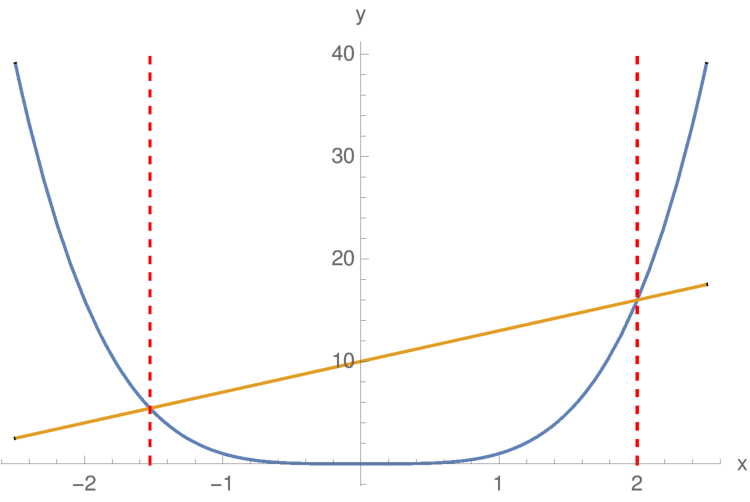
\includegraphics[width=0.9\linewidth]{convex_function.pdf}
\caption{\label{fig:convex}A chord showing convexity of the function $x^4$.} 
\end{figure}

\subsection{Convex optimisation}
\noindent A \textit{convex optimisation problem} has three components:
\begin{itemize}
\item a convex \textit{objective function} $f_0(x)$,
\item $m$ convex \textit{inequality constraint functions} $f_i(x)$,
\item $k$ convex \textit{equality constraint functions} $g_j(x)$, 
\end{itemize}
where $f,g: \mathbb{R}^n \rightarrow \mathbb{R}$ \cite[p.141]{cvxpybook}. We seek an optimum, $x^*\in \mathbb{R}^n$, where $f_0(x^*)$ is a minimum. Formally the problem is defined as:
\begin{align} \label{eq:cvxdefn}
&\text{minimise } && f_0(x) & \nonumber &\\
&\text{subject to } && f_i(x) \leq 0,\quad & i\in \{1,..,m\}\nonumber &\\
& && g_{j}(x)=0,\quad & j\in \{1,...,k\} &.
\end{align}

Any local optimum $x^*$ for a convex optimisation problem is also a global optimum \cite[pp.138-139]{cvxpybook}, however an optimum may not be unique.

\subsection{Disciplined convex programming}
\noindent In order to solve convex optimisation problems, we used \texttt{cvxpy}, a symbolic programming module for \textit{Python}\cite{cvxpy}. It uses a set of rules, called \textit{disciplined convex programming} (DCP), to determine whether a function is convex. This is implemented using predefined classes containing functions with their curvature and sign, and using general composition theorems from convex analysis \cite{dcp}. If DCP rules can be applied then interior point methods guarantee an optimal solution.

\section{Example: power minimisation in communications}
\noindent To demonstrate the applicability of \texttt{cvxpy} to  a real-world example, we consider a system of $n$ transmitters each of power $p_i$ and $m$ receivers, all in $2$D Euclidean space\cite{shannon1949}. In this problem we are constrained to having a minimum signal-to-interference-plus-noise ratio (SINR) at each receiver; the strength of the desired signal, $S$, relative to the interference power, $I$, plus the background noise, $\sigma$, at a receiver. How can we minimise the total power consumption, $P$, of transmitters, yet achieve this minimum SINR, $\gamma_0$, for all receivers? This question is relevant to telecoms companies who want to offer a service at a minimum quality standard. We formulate the problem with a given square path gain matrix, $G$, background noise level $\sigma$ and a maximum power constraint $P_{\text{max}}$ of each transmitter:
\begin{align*}
&\underset{p}{\text{minimise}} \quad &&\sum_j p_j\\
&\text{subject to} \quad &&p_j \leq P_{\max}\\
& \quad &&p_j \geq 0\\
& \quad &&\gamma_i \geq \gamma_0.&&
\end{align*}

The desired signal for receiver $i$ is $S_i = G_{ik}p_k$, while the interference at $i$ is $I_i = \sum_{j\neq k}G_{ij}p_j$. However DCP does not allow division of the optimisation variable $p_i$ so  
\begin{equation*}
  \gamma_i \geq \gamma_0\Longleftrightarrow  \frac{S_i}{\sigma_i + I_i}\geq \gamma_0, \quad \forall i
\end{equation*}
was rearranged to,
\begin{equation*}
S_i-\gamma_0(\sigma_i + I_i)\geq 0, \quad \forall i
\end{equation*} which is affine, and hence a DCP function.

\subsection{Path gain}
\noindent The path gain $G_{ij}$ represents the proportion of power that reaches receiver $i$ from transmitter $j$. Supposing that the desired signal to receiver $i$ is from transmitter $k$, the power received is,
\begin{equation}
p_{ik}^{\text{rec}} = G_{ik}p_k.
\end{equation}
Denoting the SINR at $i$ by $\gamma_i$, we have
\begin{equation}
\gamma_i = \frac{G_{ik}p_k}{\sigma_i+\sum_{j\neq k}G_{ij}p_j}
=\frac{S_i}{\sigma_i+I_i}.
\end{equation}
In a physical context, the path gain from transmitter $j$ to receiver $i$, as shown in Fig.~\ref{fig:pathgain}, will depend on the distance, $d_{ij}$ between them. Assuming isotropic propagation from each transmitter, the fraction of power from $j$ that reaches $i$ is:
\begin{equation}
G_{ij} = k_i/d_{ij}^\alpha
\end{equation}
where $\alpha$ is the pathloss coefficient and $k$ is a proportionality constant specific to the receiver $i$.  For free space $\alpha = 2$, while in urban environments $\alpha \sim 3.5$ \cite{hata1980}. Further physical complexities, such as the stochastic effects from Rayleigh fading can be easily incorporated.

\begin{figure}[H]
\centering
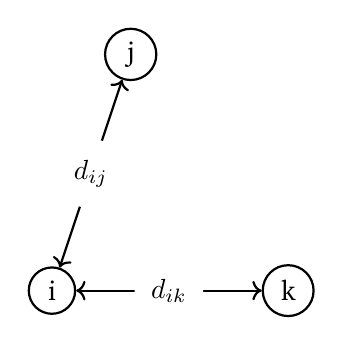
\begin{tikzpicture}
\begin{scope}[every node/.style={circle,thick,draw}]
    \node (A) at (0,0) {i};
    \node (B) at (1,3) {j};
    \node (C) at (3,0) {k};
\end{scope}
\begin{scope}[
	every node/.style={fill=white,circle},
    every edge/.style={draw=black, thick}]
    \path [<->] (A) edge node {$d_{ik}$} (C);
    \path [<->] (B) edge node {$d_{ij}$} (A);
    %\path [<->] (C) edge node {$1$} (B);
\end{scope}
\end{tikzpicture}
\caption{\label{fig:pathgain}Path lengths between receiver $i$ and transmitters $j$ and $k$.}
\end{figure}

\subsection{Example code}
\noindent To indicate the brevity of code implementation in \texttt{cvxpy} we show a minimal working example below: \lstinputlisting[language=Python,mathescape=true]{minimisePgivenSINR.py}

\section{Outlook}
\noindent The authors hope that this article shows the utility of \texttt{cvxpy} for simple `toy' problems of real-world relevance. We believe it is an invaluable resource for researchers wanting to test the applicability of convex optimisation in new fields. 

The module could also be easily incorporated into a course on optimisation, providing students with an accessible environment to practise techniques for convex optimisation. Full code for other communication examples can be found at https://github.com/cvxgrp/cvxpy/\\tree/master/examples/communications.

%While all problems that can be written in DCP are convex, not all convex problems of interest can be written in DCP.  Over time, the library of available DCP functions in \texttt{cvxpy} has grown, increasing the scope of convex optimisation problems that \texttt{cvxpy} can solve.  This expansion of scope of \texttt{cvxpy} is ongoing, with version 1.0 under development and expected in the near future.

%\section{Further Work}
%While many problems are convex, others fall into a similar category of being \textit{quasi-convex}.  A quasi-convex function $f$ is one for which $\textbf{dom} f$ and every sublevel set of $f$ is convex.  An example of this is shown in Figure [?].  Quasi-convex problems cannot be solved directly using convex optimisation solvers, however the feasibility of a sublevel set can be checked.  This feasibility check can be used as a bisection method to find the solution.  A more thorough discussion of quasi-convex problems can be found in \cite{cvxpybook}chapter?.

%\section{Further applications}
\subsection*{Acknowledgements}
We would like to thank S.~Johnson from MathSys and S.~Diamond for helpful discussions. 

\vspace{0.2cm}
%\section{Links \& references}
\bibliography{articleBib} 
\bibliographystyle{plain}

%\item DCP analyser http://dcp.stanford.edu/analyzer
% -----
\end{document}
